\section{Large Language Models}
\label{sec_review}
This section reviews LLMs, briefly describing their architectures, training objectives, pipelines, datasets, and fine-tuning details.      
\subsection{Pre-Trained Models}
\subsubsection{T5~\cite{T5}}
An encoder-decoder model trained on the Colossal Clean Crwal Corpus (C4) dataset with a unified text-to-text training for all NLP problems, shown in Figure~\ref{t5_image}. The model differs from the traditional transformer model~\cite{Transformers}. These changes include no bias in layer normalization, using relative positional embedding, and placing layer normalization outside the residual path. The masked language modeling is used as a pre-training objective where spans (consecutive tokens) were replaced with a single mask instead of separate masks for each token. This type of masking speeds up the training as it produces shorter sequences. After pre-training, the model is fine-tuned using adapter layers~\cite{LMAdapter} for downstream tasks.
\begin{figure}[tbp]
\centering
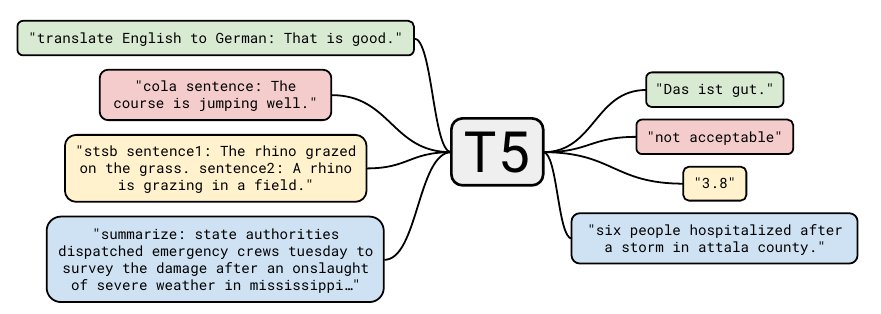
\includegraphics[width=1\columnwidth]{Figure/T5.png}
\caption{Unified text-to-text training example, source image from~\cite{T5}.}
\label{t5_image}
\end{figure}

\subsubsection{mT5~\cite{mT5}}
A multilingual T5 model~\cite{T5} trained on the mC4 dataset with 101 languages. The dataset is extracted from the public common crawl scrape. The model uses GeGLU activation and trains with a vocab size of 250,000 to cover multiple languages. To avoid over-fitting or under-fitting for a language, mT5 employs a data sampling procedure to select samples from all languages. The paper suggests using a small amount of pre-training datasets, including all languages when fine-tuning for a task using English language data. This allows the model to generate non-English outputs.  
%$p(L) \propto \mid L \mid^\alpha$, where $p(L)$ is sampling probability, $L$ is language sampling count, and $\alpha$ controls the sampling probability

\subsubsection{PanGu-$\alpha$~\cite{PanGU_alpha}}
An autoregressive model trained on 1.1TB Chinese data collected from Common Crawl, e-Books, encyclopedia, etc. Additional to the standard transformer model, it has a query layer after stacked transformer layers, example shown in Figure~\ref{pangu_alpha_image}. The purpose of the query layer is to predict the next token. Its structure is similar to the transformer layer but with an additional embedding for the next position in the attention mechanism, given in Eq.~\ref{PanGu_alpha_eq}. The model is trained using MindSpore with five-dimensional parallelism, i.e., data parallelism, op-level model parallelism, pipeline model parallelism, optimizer parallelism, and rematerialization. 
\begin{equation}
a = p_nW_h^qW_h^kTH_L^T
\label{PanGu_alpha_eq}
\end{equation}

\begin{figure}[tbp]
\centering
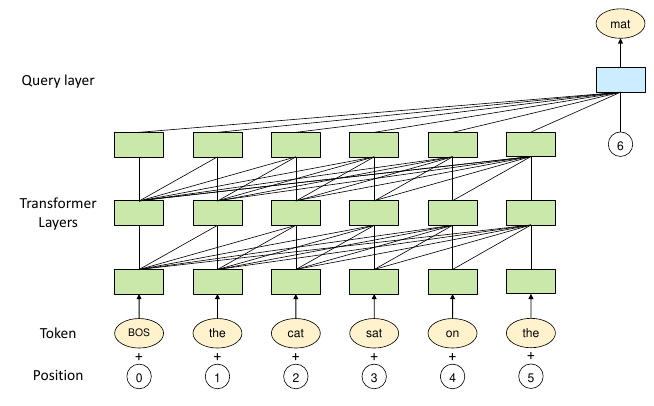
\includegraphics[width=1\columnwidth]{Figure/PanGU_alpha.png}
\caption{The image is the article of~\cite{PanGU_alpha}, showing an example of PanGu-$\alpha$ architecture.}
\label{pangu_alpha_image}
\end{figure}


\subsubsection{CPM-2~\cite{CPM-2}}
Cost-efficient Pre-trained language Models (CPM-2) pre-trains bilingual (English and Chinese) 11B and 198B mixture-of-experts (MoE) models on the WuDaoCorpus~\cite{WuDaoCorpus} dataset. It has an encoder-decoder architecture with a bidirectional encoder and a unidirectional decoder. The tokenization process removes \enquote{\_} white space tokens in the sentencepiece tokenizer. The models are trained with knowledge inheritance, starting with only the Chinese language in the first stage and then adding English and Chinese data. This trained model gets duplicated multiple times to initialize the 198B MoE model. Moreover, to use the model for downstream tasks, CPM-2 experimented with both complete fine-tuning and prompt fine-tuning as in~\cite{LMAdapted} where only prompt-related parameters are updated by inserting prompts at various positions, front, middle, and back. CPM-2 also proposes INFMOE, a memory-efficient framework with a strategy to dynamically offload parameters to the CPU for inference at a 100B scale. It overlaps data movement with inference computation for lower inference time.   

\subsubsection{CodeGen~\cite{CodeGen}}
CodeGen has similar architecture to the PaLM~\cite{PaLM}, i.e., parallel attention, MLP layers, and RoPE embeddings. The model is trained on both natural language and programming language data sequentially (trained on the first dataset, then the second and so on) on the following datasets 1) PILE, 2) BIGQUERY and 3) BIGPYTHON. CodeGen proposed a multi-step approach to synthesizing code. The purpose is to simplify the generation of long sequences where the previous prompt and generated code are given as input with the next prompt to generate the next code sequence. CodeGen opensource a Multi-Turn Programming Benchmark (MTPB) to evaluate multi-step program synthesis.   

\subsubsection{GPT-NeoX-20B~\cite{GPT_NeoX}}
An auto-regressive model that largely follows GPT-3 with a few deviations in architecture design, trained on the Pile dataset without any data deduplication. GPT-NeoX has parallel attention and feed-forward layers in a transformer block, given in Eq.~\ref{GPT-NeoX-20B_eq}, that increases throughput by 15\%. It uses rotary positional embedding~\cite{su2021roformer}, applying it to only 25\% of embedding vector dimension as in~\cite{GPT_J_6B}. This reduces the computation without performance degradation. Opposite to GPT-3, which uses dense and sparse layers, GPT-NeoX-20B uses only dense layers. The hyperparameter tuning at this scale is difficult; therefore, the model chooses hyperparameters from the method~\cite{GPT-3} and interpolates values between 13B and 175B models for the 20B model. The model training is distributed among GPUs using both tensor and pipeline parallelism.   
\begin{equation}
x + Attn(LN_1(x)) + FF(LN_2(x))
\label{GPT-NeoX-20B_eq}
\end{equation}

\subsubsection{UL2~\cite{UL2}}
An encoder-decoder architecture trained using a mixture of denoisers (MoD) objectives. Denoisers include 1) R-Denoiser: a regular span masking, 2) S-Denoiser: which corrupts consecutive tokens of a large sequence and 3) X-Denoiser: which corrupts a large number of tokens randomly. During pre-training, UL2 includes a denoiser token from ${R, S, X}$ to represent a denoising setup. It helps improve fine-tuning performance for downstream tasks that bind the task to one of the upstream training modes. This MoD style of training outperforms the T5 model on many benchmarks.   

\subsubsection{OPT~\cite{OPT}}
It is a clone of GPT-3, developed with the intention to open-source a model that replicates GPT-3 performance. The model was trained using RoBERTa, The Pile, and PushShift.io Reddit datasets. Training of OPT employs dynamic loss scaling ~\cite{S_mixed_precision} and restarts from an earlier checkpoint with a lower learning rate whenever loss divergence is observed. Overall, the performance of OPT-175B models is comparable to the GPT3-175B model.

\subsubsection{GLM-130B~\cite{GLM-130B}}
GLM-130B is a bilingual (English and Chinese) model trained using an auto-regressive mask infilling pre-training objective similar to the GLM~\cite{GLM}. This training style makes the model bidirectional as compared to GPT-3, which is unidirectional. Opposite to the GLM, the training of GLM-130B includes a small amount of multi-task instruction pre-training data (5\% of the total data) along with the self-supervised mask infilling. To stabilize the training, it applies embedding layer gradient shrink. 

\subsubsection{BLOOM~\cite{BLOOM}}
A causal decoder model trained on ROOTS corpus with the aim of open-sourcing an LLM. The architecture of BLOOM is shown in Figure~\ref{bloom_image}, with differences like ALiBi positional embedding, an additional normalization layer after the embedding layer as suggested by the bitsandbytes\footnote{https://github.com/TimDettmers/bitsandbytes} library. These changes stabilize training with improved downstream performance. 

\begin{figure}[tbp]
\centering
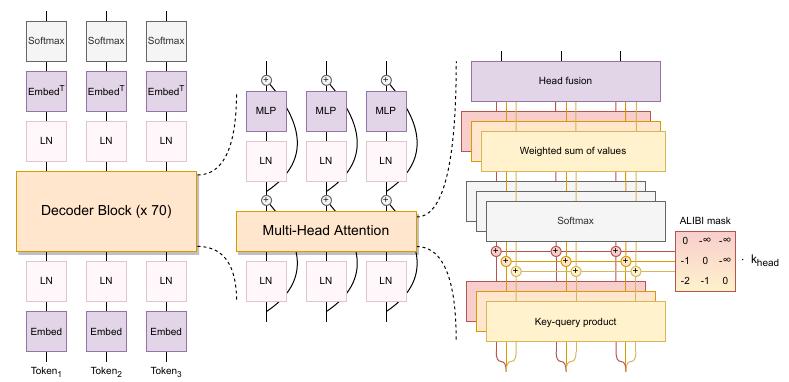
\includegraphics[width=1\columnwidth]{Figure/BLOOM.png}
\caption{The BLOOM architecture example sourced from~\cite{BLOOM}.}
\label{bloom_image}
\end{figure}

\subsubsection{Galactica~\cite{galactica}}
A large curated corpus of human scientific knowledge with 48 million papers, textbooks, lecture notes, millions of compounds and proteins, scientific websites, encyclopedias, and more are trained using metaseq library3, which is built on PyTorch and fairscale~\cite{fairscale}. The model wraps reasoning datasets with $<work>$ token to provide step-by-step reasoning context to the model, which has been shown to improve the performance on reasoning tasks.

\subsubsection{GPT-3}
The architecture of GPT-3 is mostly the same as GPT-2~\cite{GPT-2} but with dense and sparse attention in transformer layers similar to the Sparse Transformer~\cite{sparse_transformer}. The model is trained on data taken from CommonCrawl, Webtext dataset, books corpora, and English-language Wikipedia. Large models can train on larger batch sizes with a lower learning rate; in order to decide the batch size during training, GPT-3 uses the gradient noise scale as in ~\cite{batch_size_selec}. Overall, GPT-3 increases model parameters to 175B showing that the performance of large language models improves with the scale and is competitive with the fine-tuned models.  

\subsubsection{Codex~\cite{codex}}
This LLM is trained on a subset of public Python Github repositories to generate code from docstrings. Computer programming is an iterative process where the programs are often debugged and updated before fulfilling the requirements. Similarly to this, Codex generates 100 versions of a program by repetitive sampling for a given description, which produces a working solution for 77.5\% of the problems passing unit tests.  Its powerful version powers Github Copilot\footnote{https://github.com/features/copilot}.  

\subsubsection{ERNIE 3.0~\cite{ernie3}}
ERNIE 3.0 takes inspiration from multi-task learning to build a modular architecture using Transformer-XL~\cite{dai2019transformer} as the backbone. The universal representation module is shared by all the tasks, which serve as the basic block for task-specific representation modules, which are all trained jointly for natural language understanding, natural language generation, and knowledge extraction. This LLM is primarily focused on the Chinese language, claims to train on the largest Chinese text corpora for LLM training, and achieved state-of-the-art in 54 Chinese NLP tasks.

\subsubsection{Jurassic-1~\cite{lieber2021jurassic}}
A pair of auto-regressive language models, including a 7B-parameter J1-Large model and a 178B-parameter J1-Jumbo model. The Jurassic-1 models are mainly structured on the Transformer decoder module~\cite{Transformers}, while the architecture modifications proposed by GPT-2~\cite{GPT-2} are also incorporated. In particular, the training vocabulary items of Jurassic-1 comprise word pieces, complete words, and multi-word expressions without any word boundaries, where possible out-of-vocabulary instances are interpreted as Unicode bytes. In practice, data collected from publicly available resources are formed in the GPT-3's data structure to train the Jurassic-1 models following the conventional self-supervised auto-regressive training objective. Compared to the GPT-3 counterparts, the Jurassic-1 models apply a more balanced depth-to-width self-attention architecture~\cite{levine2020limits} and an improved tokenizer for a faster prediction based on broader resources, achieving a comparable performance in zero-shot learning tasks and a superior performance in few-shot learning tasks given the ability to feed more examples as a prompt.

\subsubsection{HyperCLOVA~\cite{hyperclova}}
The architecture is the same as that of GPT3~\cite{GPT-3} with morphene aware byte level encoding tokenization step. A large Korean-centric corpus gathered from various sources (see table for details) is trained using Megatron LM. Prompt-based tuning is also applied to enhance performance on downstream tasks. The main objective of training this model is to see how the non-English language model fares compared to universally found English-based LMs.

\subsubsection{Yuan 1.0~\cite{wu2021yuan}}
A large singleton language model with 245B parameters. The Yuan 1.0 is structured as a Transformer~\cite{Transformers}. A Chinese corpus with 5TB of high-quality text is created to train Yuan 1.0 model, where the raw data is collected from Internet resources. A Massive Data Filtering System (MDFS) built on Spark is developed to process the raw data via coarse and fine filtering techniques. To speed up the training of Yuan 1.0 with the aim of saving energy expenses and carbon emissions, a collaborative design of model architecture and large-scale distributed training is introduced. In practice, the Yuan 1.0 model performs well on text classification, Winograd Schema, natural language inference, and reading comprehension tasks.

\subsubsection{Gopher~\cite{gopher}}
It is the largest of six causal decoder LLMs trained on the subsets of MassiveWeb, Books, C4, News, GitHub, and Wikipedia samples from high-quality curated MassiveText. The model is a modified version of Transformer architecture used in~\cite{GPT-2}. The Gopher family of models ranges from 44M to 280B parameters in size to study the effect of \textit{scale} on the LLMs performance. The 280B model beats GPT-3~\cite{GPT-3}, Jurrasic-1~\cite{lieber2021jurassic}, MT-NLG~\cite{mtnlg}, and others on 81\% of the evaluated tasks.

\subsubsection{ERNIE 3.0 TITAN~\cite{ernie3titan}}
ERNIE 3.0 Titan extends ERNIE 3.0 by training a larger model with 26x the number of parameters of the latter. This bigger model outperformed other state-of-the-art models in 68 NLP tasks. LLMs produce text with incorrect facts. In order to have control of the generated text with factual consistency, ERNIE 3.0 Titan adds another task, \textit{Credible and Controllable Generations}, to its multi-task learning setup. It introduces additional self-supervised adversarial and controllable language modeling losses to the pre-training step, which enables ERNIE 3.0 Titan to beat other LLMs in their manually selected Factual QA task set evaluations.

\subsubsection{GLaM~\cite{du2022glam}}
Generalist Language Model (GLaM) represents a family of language models using a sparsely activated mixture-of-experts (MoE) structure~\cite{shazeer2017outrageously,fedus2022switch}. Specifically, the architecture of GLaM is derived from a Decoder-only Transformer~\cite{Transformers}. To gain more model capacity while reducing computation, the experts are sparsely activated where only the best two experts are used to process each input token. The largest GLaM model, GLaM (64B/64E), is about 7$\times$ larger than GPT-3~\cite{GPT-3}, while only a part of the parameters is activated per input token. To effectively compare with GPT-3, the evaluation of GLaM follows the similar zero, one, and few-shot learning protocols as in GPT-3. Specifically, the largest GLaM (64B/64E) model achieves better overall results while consuming only one-third of GPT-3's training energy.

\subsubsection{LaMDA~\cite{thoppilan2022lamda}}
A family of Transformer-based neural language models for dialog ranging from 2B to 137B parameters. The model architecture of LaMDA follows a decoder-only Transformer~\cite{Transformers} language model. LaMDA is pre-trained on public dialog data, public dialog utterances, and public web documents. Particularly, more than 90\% of the pre-training data is in English. Particularly, LaMDA aims to produce responses that exhibit high levels of quality, safety, and groundedness. To achieve this, discriminative and generative fine-tuning techniques are incorporated to enhance the model's safety and quality aspects. As a result, the LaMDA models can be utilized as a general language model performing various tasks.

\subsubsection{MT-NLG~\cite{mtnlg}}
A causal decoder transformer trained on two snapshots of Common Crawl along with some other datasets given in table \ref{datasets}. MT-NLG uses 8-way tensor slicing by Megatron for memory efficiency and 35-way pipeline parallelism using DeepSpeed for compute efficiency to train a 530B model, roughly 3$\times$ GPT-3 model parameters. This model beats GPT-3 on a number of evaluations.

\subsubsection{AlphaCode~\cite{li2022competition}}
A set of large language models designed for competition-level code generation tasks. Basically, the AlphaCode models follow an encoder-decoder transformer architecture~\cite{Transformers} ranging from 300M to 41B parameters. Moreover, the multi-query attention~\cite{shazeer2019fast} is applied to reduce memory and cache costs. Since competitive programming problems highly require deep reasoning and an understanding of complex natural language algorithms, the AlphaCode models are pre-trained on filtered GitHub code in popular languages and then fine-tuned on a new competitive programming dataset named CodeContests. Particularly, the CodeContests dataset mainly contains problems, solutions, and test cases collected from the Codeforces platform\footnote{https://codeforces.com/}. In practice, standard language modeling objectives are used for the pre-training on GitHub code data, while GOLD~\cite{pang2020text} with tempering~\cite{dabre2020softmax} serve as the training objective for the fine-tuning on CodeContests data. To evaluate the performance of AlphaCode, simulated programming competitions are hosted on the Codeforces platform: overall, AlphaCode ranks at the top 54.3\% among over 5000 competitors, where its Codeforces rating is within the top 28\% of recently participated users.

\subsubsection{Chinchilla~\cite{chinchilla}}
A causal decoder trained on the same dataset as the Gopher~\cite{gopher} but with a little different data sampling distribution (sampled from MassiveText). The model architecture is similar to the one used for Gopher, with the exception of AdamW optimizer instead of Adam. Chinchilla identifies the relationship that model size should be doubled for every doubling of training tokens. Over 400 language models ranging from 70 million to over 16 billion parameters on 5 to 500 billion tokens are trained to get the estimates for compute-optimal training under a given budget. The authors train a 70B model with the same compute budget as Gopher (280B) but with 4 times more data. It outperforms Gopher~\cite{gopher}, GPT-3~\cite{GPT-3}, and others on various downstream tasks, after fine-tuning. 


\subsubsection{PaLM}
A causal decoder model trained on a dataset of 780B tokens collected from webpages, books, Wikipedia, news, and others, given in Table~\ref{datasets}. The PaLM has parallel attention and feed-forward layers similar to Eq.~\ref{GPT-NeoX-20B_eq}, speeding up training 15 times faster. Additional changes to the conventional transformer model include SwiGLU activation, RoPE embeddings, multi-query attention that saves computation cost during decoding, and shared input-output embeddings. During training, loss spiking was observed, and to fix it, model training was restarted from a 100 steps earlier checkpoint by skipping 200-500 batches around the spike. Moreover, the model was found to memorize around 2.4\% of the training data at the 540B model scale, whereas this number was lower for smaller models.   

\subsubsection{AlexaTM~\cite{soltan2022alexatm}}
The first multilingual sequence-to-sequence model (20B parameter) is capable of in-context learning. The pre-training data is collected from Wikipedia and mC4 dataset~\cite{mT5} covering 12 programming languages. To enable the AlexaTM 20B model to perform on both spoken and written cases, all data is converted into spoken format via a written-to-spoken formatter. In addition to pre-training on the denoising task, an extra Causal Language Modeling (CLM) task is performed for 20\% of the time to help the model with efficient in-context learning. In practice, the model is asked to continue the input instead of denoising the input once a special CLM token is attached to the beginning of the input.

\subsubsection{Sparrow~\cite{glaese2022improving}}
An information-seeking dialogue agent is trained to gain more helpfulness and correctness with less harm. Two additions are proposed to help human raters judge agent behavior: the first is the specific natural language rules that need raters to rate separately, and the second is to make the agent show proof from sources that support factual claims when collecting opinions about the model's statements. The architecture of the Sparrow models is based on Dialogue Prompted Chinchila 70B~\cite{chinchilla}. Human data is collected for rule violations and per-turn response preferences, which mainly aims to train preference reward models (preference RMs) and a rule reward model (rule RM). In practice, reinforcement learning with advantage actor-critic (A2C)~\cite{mnih2016asynchronous} is used to train the initialized Chinchilla model; the rule RM estimated rule violation rate and the preference RMs estimated per-turn response preferences are jointly optimized. Given experimental data, Sparrow's evidence can support the sampled response for factual questions 78\% of the time. Moreover, Sparrow is highly resistant to human adversarial probing since it only violates the defined rules 8\% of the time when probed.

\subsubsection{U-PaLM~\cite{U-PaLM}}
This method trains PaLM for 0.1\% additional compute with UL2 (also named as UL2Restore) objective~\cite{UL2} using the same dataset and outperforms baseline significantly on various NLP tasks, including zero-shot, few-shot, commonsense reasoning, CoT, etc. Training with UL2R involves converting a causal decoder PaLM to a non-causal decoder PaLM and employing 50\% sequential denoising, 25\% regular denoising, and 25\% extreme denoising loss functions.

\subsubsection{LLaMA~\cite{touvron2023llama}}
A set of foundation language models varying from 7B to 65B parameters. The overall architecture of LLaMA follows the Transformer~\cite{Transformers}, while a few subsequently proposed improvements of normalization~\cite{rmsnorm}, activation~\cite{shazeer2020glu}, and positional embedding~\cite{su2021roformer} operations are incorporated for better performances. About 67\% of LLaMA's pre-training data is collected from English CommonCrawl following the CCNet method~\cite{wenzek2019ccnet}. LLaMA and the associated variants are widely used for parameter-efficient tuning, especially for instruction following tasks.

\subsubsection{PanGu-$\Sigma$~\cite{PanGu_sigma}}
An autoregressive model with parameters copied from PanGu-$\alpha$ and extended to a trillion scale with Random Routed Experts (RRE), the architectural diagram is shown in Figure~\ref{pangu_sigma_image}. RRE is similar to the MoE architecture, with distinctions at the second level, where tokens are randomly routed to experts in a domain instead of using a learnable gating method. The model has bottom layers densely activated and shared across all domains, whereas top layers are sparsely activated according to the domain. This training style allows extracting task-specific models and reduces catastrophic forgetting effects in case of continual learning. 

\begin{figure}[tbp]
\centering
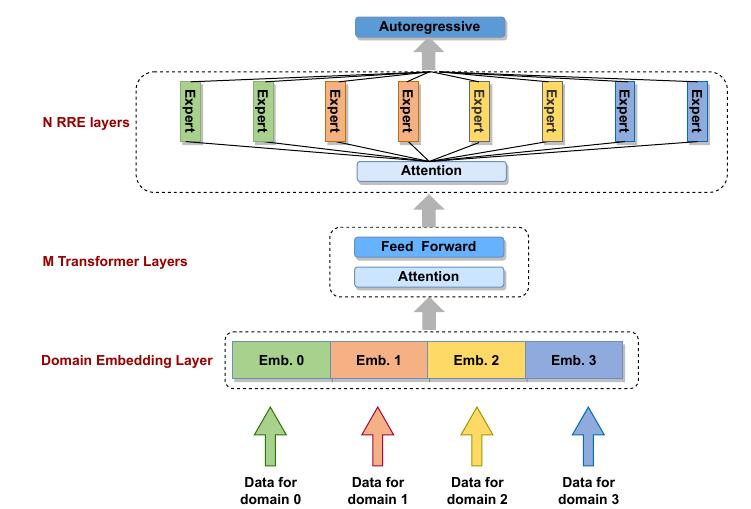
\includegraphics[width=1\columnwidth]{Figure/pangu_sigma.png}
\caption{This example illustrates the PanGu-$\sum$ architecture, as depicted in the image sourced from~\cite{PanGu_sigma}.}
\label{pangu_sigma_image}
\end{figure}


\begin{table*}[!tbhp]

%\renewcommand\tabcolsep{1pt}
\caption{Some of the critical findings and crucial discoveries of each \emph{pre-trained} Large Language Model.}
%\caption{Important findings of pre-trained LLMs}
\begin{tabular}{lc}
\hline \hline
\rowcolor{gray!50} Models & Findings \& Insights\\ \hline \hline
T5 & \begin{tabular}{c} 
\multicolumn{1}{p{15cm}}{\begin{itemize}
\item Encoder and decoder with shared parameters perform equivalently when parameters are not shared
\item Fine-tuning model layers (adapter layers) work better than the conventional way of training on only classification layers
\end{itemize}}
\end{tabular}  \\ \cline{2-2}%\hline

mT5 & \begin{tabular}{c}
\multicolumn{1}{p{15cm}}{\begin{itemize}
\item Large multi-lingual models perform equivalently to single language models on downstream tasks. However, smaller multi-lingual models perform worse
\end{itemize}}
\end{tabular}    \\ \cline{2-2}%\hline

CPM-2 & \begin{tabular}{c}
\multicolumn{1}{p{15cm}}{\begin{itemize}
\item Prompt fine-tuning requires updating very few parameters while achieving performance comparable to full model fine-tuning 
\item Prompt fine-tuning takes more time to converge as compared to full model fine-tuning 
\item Inserting prompt tokens in-between sentences can allow the model to understand relations between sentences and long sequences
\item In an analysis, CPM-2 finds that prompts work as a provider (additional context) and aggregator (aggregate information with the input text) for the model
\end{itemize}}
\end{tabular}  \\ \cline{2-2}%\hline

PanGu-$\alpha$ & \begin{tabular}{c}
\multicolumn{1}{p{15cm}}{\begin{itemize}
\item LLMs are good at a few shot capabilities
\end{itemize}}
\end{tabular} \\ \cline{2-2}%\hline

CodeGen & \begin{tabular}{c}
\multicolumn{1}{p{15cm}}{\begin{itemize}
\item Multi-step prompting for code synthesis leads to a better user intent understanding and code generation
\end{itemize}}
\end{tabular}    \\ \cline{2-2}%\hline

GPT-NeoX-20B & \begin{tabular}{c}
\multicolumn{1}{p{15cm}}{\begin{itemize}
\item Parallel attention + FF layers speed-up training 15\% with the same performance as with cascaded layers
\item Initializing feed-forward output layers before residuals with scheme in~\cite{Mesh_Transformer_JAX} avoids activations from growing with increasing depth and width
\item Training on Pile outperforms GPT-3 on five-shot 
\end{itemize}}
\end{tabular}    \\ \cline{2-2}%\hline

UL2 & \begin{tabular}{c}
\multicolumn{1}{p{15cm}}{\begin{itemize}
\item Mode switching training enables better performance on downstream tasks
\item CoT prompting outperforms standard prompting for UL2  
\end{itemize}}
\end{tabular}    \\ \cline{2-2}%\hline

OPT & \begin{tabular}{c}
\multicolumn{1}{p{15cm}}{\begin{itemize}
\item Restart training from an earlier checkpoint with a lower learning rate if loss diverges
\item Model is prone to generate repetitive text and stuck in a loop
\end{itemize}}
\end{tabular}    \\ \cline{2-2}%\hline

GLM-130B &  \begin{tabular}{c}
\multicolumn{1}{p{15cm}}{\begin{itemize}
\item Pre-training data with a small proportion of multi-task instruction data improves the overall model performance
\end{itemize}}
\end{tabular}    \\ \cline{2-2}%\hline

BLOOM & \begin{tabular}{c}
\multicolumn{1}{p{15cm}}{\begin{itemize}
\item None
\end{itemize}}
\end{tabular}  \\ \cline{2-2}%\hline

Galactica & \begin{tabular}{c}
\multicolumn{1}{p{15cm}}{\begin{itemize}
\item Galactica's performance has continued to improve across validation set, in-domain, and out-of-domain benchmarks, even with multiple repetitions of the corpus, which is superior to existing research on LLMs.
\item A working memory token approach can achieve strong performance over existing methods on mathematical MMLU and MATH benchmarks. It sets a new state-of-the-art on several downstream tasks such as PubMedQA (77.6\%) and MedMCQA dev (52.9\%).
\end{itemize}}
\end{tabular}    \\ \cline{2-2}%\hline

GPT-3 & \begin{tabular}{c}
\multicolumn{1}{p{15cm}}{\begin{itemize}
\item Few-shot performance of LLMs is better than the zero-shot, suggesting that LLMs are meta-learners
\end{itemize}}
\end{tabular}    \\ \cline{2-2}%\hline

Codex & \begin{tabular}{c}
\multicolumn{1}{p{15cm}}{\begin{itemize}
\item This LLM focuses on code evaluations and introduces a novel way of selecting the best code samples.
\item The results indicate it is possible to accurately select code samples using heuristic ranking in lieu of a detailed evaluation of each sample, which may not be feasible or feasible in some situations.
\end{itemize}}
\end{tabular}    \\ \cline{2-2}%\hline

ERNIE 3.0 & \begin{tabular}{c}
\multicolumn{1}{p{15cm}}{\begin{itemize}
\item ERNIE 3.0 shows that a modular LLM architecture with a universal representation module and task-specific representation module helps in finetuning phase.
\item Optimizing the parameters of a task-specific representation network during the fine-tuning phase is an efficient way to take advantage of the powerful pretrained model.
\end{itemize}}
\end{tabular}    \\ \cline{2-2}%\hline

Jurassic-1 & \begin{tabular}{c}
\multicolumn{1}{p{15cm}}{\begin{itemize}
\item The performance of an LLM is highly related to the network size.
\item To improve runtime performance, more operations can be performed
in parallel (width) rather than sequentially (depth).
\item To efficiently represent and fit more text in the same context length, the model uses a larger vocabulary to train a SentencePiece tokenizer without restricting it to word boundaries. This tokenizer improvement can further benefit few-shot learning tasks.
\end{itemize}}
\end{tabular}    %\\ \cline{2-2}%\hline

\\ \hline
\end{tabular}%
\vspace{2mm}
\begin{flushright}
Table Continued on Next Page 
\end{flushright}
 \label{tab:pre_trained_findings}
\end{table*}

%\clearpage
%\pagebreak

\begin{table*}[!tbhp]
%\ContinuedFloat
%\caption{(Continued on next page)}
\begin{tabular}{lc}
\hline \hline
\rowcolor{gray!50}Models & Findings  \& Insights\\ \hline \hline

HyperCLOVA & \begin{tabular}{c}
\multicolumn{1}{p{15cm}}{\begin{itemize}
\item By employing prompt-based tuning, the performances of models can be improved, often surpassing those of state-of-the-art models when the backward gradients of inputs are accessible.
\end{itemize}}
\end{tabular}    \\ \cline{2-2}%\hline

Yuan 1.0 & \begin{tabular}{c}
\multicolumn{1}{p{15cm}}{\begin{itemize}
\item The model architecture that excels in pre-training and fine-tuning cases may exhibit contrasting behavior in zero-shot and few-shot learning.
\end{itemize}}
\end{tabular}    \\ \cline{2-2}%\hline

Gopher & \begin{tabular}{c}
\multicolumn{1}{p{15cm}}{\begin{itemize}
\item Relative encodings enable models to be evaluated for longer sequences than those on which it was trained.
\end{itemize}}
\end{tabular}    \\ \cline{2-2}%\hline

ERNIE 3.0 Titan & \begin{tabular}{c}
\multicolumn{1}{p{15cm}}{\begin{itemize}
\item This LLM builds on top of ERNIE 3.0 and add a self-supervised adversarial loss to distinguish whether a text is generated or the original one. 
\item This distinction ability between real and generate text improves the LLM's performance as compared to ERNIE 3.0.
\end{itemize}}
\end{tabular}    \\ \cline{2-2}%\hline

GLaM & \begin{tabular}{c}
\multicolumn{1}{p{15cm}}{\begin{itemize}
\item The feed-forward component of each Transformer layer can be replaced with a mixture-of-experts (MoE) module consisting of a set of independent feed-forward networks (\emph{i.e.}, the `experts'). By sparsely activating these experts, the model capacity can be maintained while much computation is saved. 
\item By leveraging sparsity, we can make significant strides towards developing high-quality NLP models while simultaneously reducing energy consumption. Consequently, MoE emerges as a robust candidate for future scaling endeavors.
\item The model trained on filtered data shows consistent better performances on both NLG and NLU tasks, where the effect of filtering is more significant on the former tasks.
\item Filtered pretraining corpora plays a crucial role in the generation capability of LLMs, especially for the downstream tasks.
\item The scaling of GLaM MoE models can be achieved by increasing the size or number of experts in the MoE layer. Given a fixed budget of computation, more experts contribute to better predictions.
\end{itemize}}
\end{tabular}    \\ \cline{2-2}% \hline

LaMDA & \begin{tabular}{c}
\multicolumn{1}{p{15cm}}{\begin{itemize}
\item The model can be fine-tuned to learn to call different external information resources and tools.
\end{itemize}}
\end{tabular}    \\ \cline{2-2}%\hline

MT-NLG & \begin{tabular}{c}
\multicolumn{1}{p{15cm}}{\begin{itemize}
\item None.
\end{itemize}}
\end{tabular} \\ \cline{2-2}%\hline

AlphaCode & \begin{tabular}{c}
\multicolumn{1}{p{15cm}}{\begin{itemize}
\item For higher effectiveness and efficiency, a transformer model can be asymmetrically constructed with a shallower encoder and a deeper decoder.
\item To achieve better performances, it is necessary to employ strategies such as massively scaling up sampling, followed by the filtering and clustering of samples into a compact set. 
\item The utilization of novel sampling-efficient transformer architectures designed to facilitate large-scale sampling is crucial.
\item Simplifying problem descriptions can effectively improve the model’s performance.
\end{itemize}}
\end{tabular}    \\ \cline{2-2}%\hline

Chinchilla & \begin{tabular}{c}
\multicolumn{1}{p{15cm}}{\begin{itemize}
\item The experiments that culminated in the development of Chinchilla determined that for optimal computation during training, the model size and the number of training tokens should be scaled proportionately: for each doubling of the model size, the number of training tokens should be doubled as well.
\end{itemize}}
\end{tabular}    \\  \cline{2-2} %\hline
PaLM &  \begin{tabular}{c}
\multicolumn{1}{p{15cm}}{\begin{itemize}
\item English-centric models produce better translations when translating to English as compared to non-English
\item Generalized models can have equivalent performance for language translation to specialized small models
\item Larger models have a higher percentage of training data memorization
\item Performance has not yet saturated even at 540B scale, which means larger models are likely to perform better
\end{itemize}}
\end{tabular}   \\ \cline{2-2}%\hline

AlexaTM & \begin{tabular}{c}
\multicolumn{1}{p{15cm}}{\begin{itemize}
\item Compared to commonly used Decoder-only Transformer models, seq2seq architecture is more suitable for training generative LLMs given stronger bidirectional attention to the context. 
\item An extra Causal Language Modeling (CLM) task can be added to benefit the model with a more efficient in-context learning, especially for few-shot learning tasks. 
\item The key to training powerful seq2seq-based LLMs lies in mixed pre-training, rather than additional multitask training.
\item Placing layernorms at the beginning of each transformer layer can improve the training stability of large models.
\end{itemize}}
\end{tabular}    \\ \cline{2-2}%\hline

Sparrow & \begin{tabular}{c}
\multicolumn{1}{p{15cm}}{\begin{itemize}
\item Reinforcement learning from multi-objective human feedback can be leveraged to train the models, in order to maximize preference rates and minimize rule violations.
\item The judgments of labelers and the alignments with defined rules can help the model generate better responses.
\item Good dialogue goals can be broken down into detailed natural language rules for the agent and the raters.
\item Constructing useful and reliable agents from generative models requires a combination of width and depth: the width aspect enables addressing the complexities of goals and topics; while the depth aspect ensures accurate handling of them.
\item The combination of reinforcement learning (RL) with reranking yields optimal performance in terms of preference win rates and resilience against adversarial probing.
\end{itemize}}
\end{tabular}    \\ \hline %\cline{2-2}



%InstructGPT & \begin{tabular}{c}
%\multicolumn{1}{p{15cm}}{\begin{itemize}
%\item InstructGPT is trained using a novel RLHF technique which produces outputs that are preferred to the outputs from its base model of GPT-3 (175B), despite having 100x fewer parameters.
%\item The human feedback step-trained models show improvements in truthfulness and reductions in toxic output generation while having minimal performance regressions on public NLP datasets
%\end{itemize}}
%\end{tabular}    \\ \hline %\hline

\end{tabular}%

\vspace{2mm}
\begin{flushright}
Table Continued on Next Page 
\end{flushright}
\end{table*}

\begin{table*}[!tbhp]
%\ContinuedFloat
%\caption{}
\begin{tabular}{lc}
\hline \hline
\rowcolor{gray!50}Model & Findings \& Insights \\ \hline \hline

U-PaLM & \begin{tabular}{c}
\multicolumn{1}{p{15cm}}{\begin{itemize}
\item Training with a mixture of denoisers outperforms PaLM when trained further for a few more FLOPs 
\item Training with a mixture of denoisers improves the infilling ability and open-ended text generation diversity
\end{itemize}}
\end{tabular}\\\cline{2-2}% \hline

LLaMA & \begin{tabular}{c}
\multicolumn{1}{p{15cm}}{\begin{itemize}
\item LLaMA is open-source and can be fine-tuned or continually pre-trained to develop new models or instruction-based tools.
\item A few optimizations are proposed to improve the training efficiency of LLaMA, such as efficient implementation of multi-head self-attention and a reduced amount of activations during back-propagation.
\item Training exclusively on public data can also achieve state-of-the-art performance.
\item A constant performance improvement is gained when scaling the model.
\item Smaller models can also realize good performances using more training data and time.  
\end{itemize}}
\end{tabular}    \\ \cline{2-2}%\hline


PanGu-$\Sigma$ & \begin{tabular}{c}
\multicolumn{1}{p{15cm}}{\begin{itemize}
\item Sparse models provide the benefits of large models at a lower computation cost
\item Randomly Routed Experts reduces catastrophic forgetting effects which in turn is essential for continual learning 
\item Randomly Routed Experts allow extracting a domain-specific sub-model in deployment which is cost-efficient while maintaining a performance similar to the original
\end{itemize}}
\end{tabular}    \\ \hline

\end{tabular}%
\end{table*}


\begin{table*}[!tbhp]
\caption{Our several key insights and findings from the study of \emph{instruction-tuned} Large Language Models. }
%\caption{Important findings of instruction-tuned LLMs}

\begin{tabular}{lccl}
\hline \hline
\rowcolor{gray!50}Models & Findings \& Insights \\ \hline \hline

T0 & \begin{tabular}{c}
\multicolumn{1}{p{15cm}}{\begin{itemize}
\item Multi-task prompting enables zero-shot generalization and outperforms baselines    
\item Even a single prompt per dataset task is enough to improve performance
\end{itemize}}
\end{tabular}\\ \cline{2-2}%\hline

WebGPT & \begin{tabular}{c}
\multicolumn{1}{p{15cm}}{\begin{itemize}
\item The answer quality of LLMs can be further improved with human feedback. 
\item To aid the model in effectively filtering and utilizing relevant information, human labelers play a crucial role in answering questions regarding the usefulness of the retrieved documents.
\item Interacting a fine-tuned language model with a text-based web-browsing environment can improve end-to-end retrieval and synthesis via imitation learning and reinforcement learning.
\item Generating answers with references can make labelers easily judge the factual accuracy of answers.%\textbf{}
\end{itemize}}
\end{tabular}    \\ \cline{2-2}%\hline

Tk-INSTRUCT & \begin{tabular}{c}
\multicolumn{1}{p{15cm}}{\begin{itemize}
\item Instruction tuning leads to a stronger generalization of unseen tasks 
\item More tasks improve generalization whereas only increasing task instances does not help 
\item Supervised trained models are better than generalized models 
\item Models pre-trained with instructions and examples perform well for different types of inputs 
\end{itemize}}
\end{tabular}    \\ \cline{2-2}%\hline


mT0 and BLOOMZ & \begin{tabular}{c}
\multicolumn{1}{p{15cm}}{\begin{itemize}
\item Instruction tuning enables zero-shot generalization to the tasks never seen before    
\item Multi-lingual training leads to even better zero-shot generalization for both English and non-English
\item Training on machine-translated prompts improves performance for held-out tasks with non-English prompts  
\item English only fine-tuning on multilingual pre-trained language model is enough to generalize to other pre-trained language tasks
\end{itemize}}
\end{tabular}    \\ \cline{2-2} 

OPT-IML & \begin{tabular}{c}
\multicolumn{1}{p{15cm}}{\begin{itemize}
\item Task size sampling to create a batch with most of the task examples is important for better performance 
\item Only example proportional sampling is not enough, training datasets/benchmarks should also be proportional for better generalization/performance
\item Fully held-out and partially supervised tasks performance improves by scaling tasks or categories whereas fully supervised tasks have no effect

\item Including small amounts i.e. 5\% of pretraining data during fine-tuning is effective 

\item Only 1\% reasoning data improves the performance, adding more deteriorates performance

\item Adding dialogue data makes the performance worse

%\item Meta training for in-context learning degrades performance??? It improves performance for other LLMs though.
\end{itemize}}
\end{tabular}    \\ \cline{2-2}%\hline



Flan & \begin{tabular}{c}
\multicolumn{1}{p{15cm}}{\begin{itemize}
\item Finetuning with CoT improves performance on held-out tasks 
\item Fine-tuning along with CoT data improves reasoning abilities 
\item CoT tuning improves zero-shot reasoning 
\item Performance improves with more tasks 
\item Instruction fine-tuning improves usability which otherwise is challenging for pre-trained models
\item Improving the model's performance with instruction tuning is compute efficient 
\item Multitask prompting enables zero-shot generalization abilities in LM
\end{itemize}}
\end{tabular}\\ \hline %\cline{2-2}
\end{tabular}%
\label{tab:instruction_tuned_findings}
\end{table*}

\begin{table*}[htbp]
\rowcolors{2}{gray!25}{white}
\begin{center}
\caption{Statistics  of  pre-trained LLMs greater than 10B parameters. Pre-training data scale (either in the number of tokens or storage size), and hardware resource costs. In this table, we only include LLMs with a public paper about the technical details. Here, \enquote{Release Time} indicates the date when the corresponding paper was officially released. \enquote{Open Source} means  that the model checkpoints can be publicly accessible. \enquote{Data Cleaning} indicates whether the data cleaning is performed or not. This includes heuristics (Heur), deduplication (Dedup), quality filtering (QF) and privacy filtering (PF).
\enquote{Training Parallelism} indicates distributed training using data parallelism (D), tensor parallelism (T), pipeline parallelism (P), model parallelism (M), optimizer parallelism (OP), and materialization (R). 
}
\label{tab:statistics_pt}
\footnotesize
%\renewcommand\tabcolsep{1pt}
%\hspace*{-5em}
\resizebox{\linewidth}{!}{
\begin{tabular}{llcrccccccccccc}
\toprule
\rowcolor{gray!50}
  &  &   &  & & &   &    & &  &  & &   \\
\rowcolor{gray!50}
\multirow{-2}{*}{\textbf{Models}} & \multirow{-2}{*}{\textbf{\begin{tabular}[c]{@{}c@{}}Release\\ Time\end{tabular}}} & \multirow{-2}{*}{\textbf{\begin{tabular}[c]{@{}c@{}}Open\\ Source\end{tabular}}} & \multicolumn{1}{c}{\multirow{-2}{*}{\textbf{\begin{tabular}[c]{@{}c@{}}Size\\ (B)\end{tabular}}}} & \multirow{-2}{*}{\textbf{\begin{tabular}[c]{@{}c@{}}Base\\ Model\end{tabular}}} & \multirow{-2}{*}{\textbf{\begin{tabular}[c]{@{}c@{}}Steps\\ Trained\end{tabular}}} & \multirow{-2}{*}{\textbf{\begin{tabular}[c]{@{}c@{}}Data/\\ Tokens\end{tabular}}} & \multirow{-2}{*}{\textbf{\begin{tabular}[c]{@{}c@{}}Data\\ Cleaning\end{tabular}}} & \textbf{Hardware} & \multirow{-2}{*}{\textbf{\begin{tabular}[c]{@{}c@{}}Training\\ Time\end{tabular}}} &  \multirow{-2}{*}{\textbf{\begin{tabular}[c]{@{}c@{}}Training\\ Parallelism\end{tabular}}} & \textbf{Library}  \\
\midrule
T5~\cite{T5}   & Oct-2019 &$\checkmark$ & 11   & -   & 1M & 1T & Heur+Dedup & 1024 TPU v3 &  & D+M & Mesh TensorFlow  \\

mT5~\cite{mT5}  & Oct-2020  &$\checkmark$  & 13    & T5  & 1M & 1T & - & -   & -  & - & - \\

{PanGu-$\alpha$}~\cite{PanGU_alpha}   & Apr-2021    &  $\checkmark$  & 200  &  -  &  260k  & 1.1TB  & Heur+Dedup &  2048 Ascend 910  & - & D+OP+P+O+R & MindSpore\\

CPM-2~\cite{CPM-2}    & Jun-2021  & $\checkmark$  & 198   & - & 1M & 2.6TB  & Dedup & - & - & D+M  & JAXFormer   \\

CodeGen~\cite{CodeGen}  & Mar-2022    &  $\checkmark$  & 16   & -  & 650k & 577B  & Heur+Dedup   & TPU v4 & - & D+M & JAXFormer  \\

GPT-NeoX-20B~\cite{black2022gpt} & Apr-2022    & $\checkmark$    & 20   & - & 150k & 825GB & None & 96 40G A100 & - & M & Megatron+DS+PyTorch     \\

UL2~\cite{UL2}  & May-2022    &  $\checkmark$   & 20   & T5  & 2M & 1T & - & 512 TPU v4  & -  & M & JAX+T5X    \\

OPT~\cite{OPT}  & May-2022    & $\checkmark$   & 175   & - &  150k  & 180B  &  Dedup   & 992 80G A100  & -  & D+T & Megatron   \\

GLM~\cite{GLM-130B}  & Oct-2022 & $\checkmark$   & 130   & - & - & 400B   & -  & 768 40G A100    & 60d  & M & -    \\

BLOOM~\cite{BLOOM}    & Nov-2022  & $\checkmark$  & 176   & -   & - & 366B & Dedup+PR  & 384 80G A100    & 105d  &  D+T+P  & Megatron+DS    \\

Galactica~\cite{galactica} & Nov-2022    & $\checkmark$ & 120   & - & 225k & 106B & Dedup  &  128 80GB A100   & -  & - & Metaseq    \\

GPT-3~\cite{GPT-3}    & May-2020   & $\times$ & 175   & - & - & 300B & -  & -   & -  & - & -       \\

Codex~\cite{codex}    & Jul-2021 & $\times$   & 12    & GPT-3 & - & 100B & Heur & -   & -  & -    & - \\

ERNIE 3.0~\cite{ernie3}    & Jul-2021  & $\times$  & 10  & - & 120k$^*$ & 375B & Heur+Dedup & 384 V100   & -  & M$^*$ & PaddlePaddle    \\

Jurassic-1~\cite{lieber2021jurassic}   & Aug-2021 & $\times$  & 178      & - & - & 300B   & -  & 800 GPU & -  & D+M+P    & Megatron+DS       \\

HyperCLOVA~\cite{hyperclova}   & Sep-2021 & $\times$   & 82 & -  & - &  300B  & Clf+Dedup+PF & 1024 A100   & 13.4d  & M  & Megatron      \\

Yuan 1.0~\cite{wu2021yuan}   & Oct-2021  & $\times$  & 245   & -  & 26k$^*$ &  180B  &  Heur+Clf+Dedup  & 2128 GPU  &  -  & D+T+P & - \\

% WebGPT~\cite{nakano2021webgpt}   & Dec-2021  &$\times$  & 175   & GPT-3   & - & -  & - & -  & -   & -  & -   \\

Gopher~\cite{gopher}   & Dec-2021 & $\times$   & 280 & ERNIE-3.0 & - & 300B   & QF+Dedup  & 4096 TPU v3 & 920h  & D+M    & JAX+Haiku        \\

ERNIE 3.0 Titan~\cite{ernie3titan}   & Dec-2021 & $\times$   & 260  & -  & - &  300B  & Heur+Dedup &  V100+Ascend 910  & -  & D+M+P+D* & PaddlePaddle  \\

GLaM~\cite{du2022glam} &Dec-2021  &$\times$    & 1200  & -   & 600k$^*$  & 600B   & Clf  & 1024 TPU v4 & -  & M & GSPMD       \\

LaMDA~\cite{thoppilan2022lamda}    & Jan-2022   & $\times$ & 137      & - & 3M & 2.81T  & Filtered  & 1024 TPU v3 & 57.7d & D+M    & Lingvo    \\

MT-NLG~\cite{mtnlg}   & Jan-2022    & $\times$   & 530   & - & - & 270B & - & 4480 80G A100   & -  & D+T+P    & Megatron+DS       \\

AlphaCode~\cite{li2022competition}    & Feb-2022  &$\times$  & 41    & -   & 205k & 967B & Heur+Dedup & TPU v4  & -  &M   & JAX+Haiku       \\

Chinchilla~\cite{chinchilla}   & Mar-2022    & $\times$    & 70   & - & - & 1.4T  & QF+Dedup  & TPUv3/TPUv4   & -  & -    & JAX+Haiku        \\

PaLM~\cite{PaLM} & Apr-2022    & $\times$ & 540 & - &  255k  & 780B  & Heur & 6144 TPU v4  & - & D+M & JAX+T5X\\

AlexaTM~\cite{soltan2022alexatm}  & Aug-2022 &$\times$   & 20  & -  & 500k  & 1.1T   & Filtered  & 128 A100    & 120d  & M & DS      \\

Sparrow~\cite{glaese2022improving}  & Sep-2022 &$\times$    & 70    & Chinchilla   & - & -  & -  & 64 TPU v3   & -  & M    & -       \\

U-PaLM~\cite{U-PaLM}   & Oct-2022    & $\times$ & 540   & PaLM & 20k & - & -   & 512 TPU v4  & 5d    & - & - \\

LLaMA~\cite{touvron2023llama}    & Feb-2023 & $\checkmark$   & 65      & - & 350k & 1.4T & Heur+Dedup   & 2048 80G A100 & 21d   & D+M & xFormers     \\

{PanGu-$\Sigma$}~\cite{PanGu_sigma}    & Mar-2023  & $\times$  & 1085 & {PanGu-$\alpha$} & -  & 329B & -  & 512 Ascend 910   & 100d  & D+OP+P+O+R & MindSpore  \\
%\multirow{-25}{*}{\begin{tabular}[c]{@{}c@{}}Closed\\ Source\end{tabular}} & \multirow{-18}{*}{\begin{tabular}[c]{@{}c@{}}Publicly\\ Available\end{tabular}} &
\bottomrule
\end{tabular}
} 
\end{center}
\end{table*}





\begin{table*}[tbp]
\rowcolors{2}{gray!25}{white}
\centering
\caption{Statistics of instruction tuned LLMs greater than 10B parameters. All abbreviations are the same as Table~\ref{tab:statistics_pt}}
\footnotesize
\resizebox{\linewidth}{!}{
\begin{tabular}{llcrccccccccccc}
\toprule
\rowcolor{gray!50}
  &  &   &  & & &   &    & &  &  & &   \\
\rowcolor{gray!50}
\multirow{-2}{*}{\textbf{Models}} & \multirow{-2}{*}{\textbf{\begin{tabular}[c]{@{}c@{}}Release\\ Time\end{tabular}}} & \multirow{-2}{*}{\textbf{\begin{tabular}[c]{@{}c@{}}Open\\ Source\end{tabular}}} & \multicolumn{1}{c}{\multirow{-2}{*}{\textbf{\begin{tabular}[c]{@{}c@{}}Size\\ (B)\end{tabular}}}} & \multirow{-2}{*}{\textbf{\begin{tabular}[c]{@{}c@{}}Base\\ Model\end{tabular}}}  & \multirow{-2}{*}{\textbf{\begin{tabular}[c]{@{}c@{}}Steps\\ Trained\end{tabular}}} & \multirow{-2}{*}{\textbf{\begin{tabular}[c]{@{}c@{}}Data/\\ Tokens\end{tabular}}} & \multirow{-2}{*}{\textbf{\begin{tabular}[c]{@{}c@{}}Data\\ Cleaning\end{tabular}}} & \textbf{Hardware} & \multirow{-2}{*}{\textbf{\begin{tabular}[c]{@{}c@{}}Training\\ Time\end{tabular}}} &  \multirow{-2}{*}{\textbf{\begin{tabular}[c]{@{}c@{}}Training\\ Parallelism\end{tabular}}} & \textbf{Library}  \\
\midrule

T0~\cite{T0}   & Oct-2021  & $\checkmark$ & 11    & T5  & -  & 250B &  - & 512 TPU v3  & 270h   & - & - \\

WebGPT~\cite{nakano2021webgpt}   & Dec-2021  &$\times$  & 175   & GPT-3   & -  & - & -  & -   & -  &  - &  -  \\

Tk-Instruct~\cite{Tk-INSTRUCT}  & Apr-2022   & $\checkmark$ & 11    & T5  & 1000  & - & - & 256 TPU v3   & 4h  & -  & Google T5   \\

mT0~\cite{mT0}  & Nov-2022  & $\checkmark$  & 13    & mT5 & -  & - & - & -  & -   & -  & - \\

OPT-IML~\cite{OPT_IML}  & Dec-2022  & $\checkmark$ & 175   & OPT & 8k  & 2B & Dedup & 128 40G A100   & - & D+T & Megatron    \\

Flan-U-PaLM~\cite{Flan}  & Oct-2022  & $\times$ & 540   & U-PaLM  & 30k  & - & -  & 512 TPU v4 & - & - & JAX+T5X  \\


%\multirow{-25}{*}{\begin{tabular}[c]{@{}c@{}}Closed\\ Source\end{tabular}} & \multirow{-18}{*}{\begin{tabular}[c]{@{}c@{}}Publicly\\ Available\end{tabular}} &
\bottomrule
\end{tabular}}
\label{tab:statistics_it}
\end{table*}




\subsection{Instruction-Tuned Models}

\subsubsection{T0}
Similar to Flan~\cite{Flan}, T0 fine-tunes the LM-adapted T5 model~\cite{LMAdapted} with multi-task instruction prompts. To train the model, T0 designs various prompt templates to convert different datasets into prompts. The model trained with explicit multi-task prompting improves zero-shot performance, outperforming models 6 to 16 times larger in size.  

\subsubsection{WebGPT~\cite{nakano2021webgpt}}
A set of fine-tuned GPT-3~\cite{GPT-3} models that can answer long-form questions in a text-based web-browsing environment. During browsing, the models must collect references to support their answers in order to exploit easier human evaluation. In addition to the Q\&A data in the ELI5 dataset~\cite{fan2019eli5}, two more types of data, \emph{demonstrations} of humans and \emph{comparisons} between two model-generated answers, are collected for training. Using human labelers' feedback on whether the retrieved information is useful to answer the given inputs, the data is tested with four usages: behavior cloning, reward modeling, reinforcement learning, and rejection sampling. Practically, the combination of behavior cloning and rejection sampling contributes to the best-performing model containing 175B parameters. To evaluate the performance of the WebGPT model, the model's answers are compared with the human demonstrators' written ones, the highest-voted answers in ELI5~\cite{fan2019eli5}, and the adversarial short-form questions and answers in the TruthfulQA~\cite{lin2021truthfulqa} dataset.

\subsubsection{Tk-INSTRUCT~\cite{Tk-INSTRUCT}}
Tk-INSTRUCT instruction fine-tunes T5 model on self-proposed SUPER-NATURALINSTRUCTIONS dataset of 1616 different NLP tasks. To analyze the generalization capabilities of Tk-INSTRUCT, the model is evaluated on unseen tasks with a few examples as ground-truth in-context instructions. The model outperforms GPT-3 and Instruct-GPT by large margins, although it is smaller in size 11B, opposite to 175B.   

\subsubsection{mT0 and BLOOMZ~\cite{mT0andBLOOMZ}}
This method fine-tunes BLOOM and T0 using a multilingual multi-task prompt dataset. It creates a new dataset named xP3, adding 46 different language datasets with new tasks not present previously in P3. Training with this dataset improves zero-shot generalization for both English and non-English. This also leads to better generalization on held-out tasks.    

\begin{figure}[!tbp]
\centering
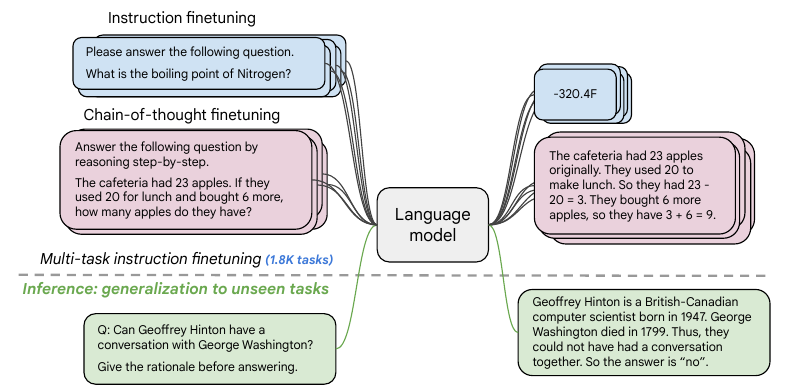
\includegraphics[width=1\columnwidth]{Figure/Flan.png}
\caption{An example image shows an instance of the Flan training paradigm, taken from~\cite{Flan}.}
\label{flan_image}
\end{figure}
\subsubsection{OPT-IML~\cite{OPT_IML}}
An instruction-tuned OPT model, trained on instruction meta-learning benchmark of 2000 NLP tasks that is a combination of 8 meta-datasets including, Super-NaturalInstructions, PromptSource, FLAN, and others as given in Table~\ref{datasets}. For computational efficiency, OPT-IML utilizes the maximum sequence length of 2048 tokens by packing multiple instances together, separated by the $<eos>$ token during training. It employs a masking mechanism to separate instances in a sequence to avoid attending tokens from different instances. Overall, OPT-IML outperforms baseline model OPT with instruction-finetuning on zero and few-shot generalization abilities.

\subsubsection{Flan~\cite{Flan}}
Fine-tuning language models (Flan), fine-tunes T5, PaLM, and UPaLM with 1836 instruction tasks taken from Muffin (80 tasks), T0-SF (193 tasks), NIV2 (1554 tasks), and CoT (taken from nine datasets), as shown in Figure~\ref{flan_image}. Instruction fine-tuning improves the model performance significantly with minimal computing, only 0.2\% of the total pre-training compute in the case of PaLM 540B. Flan also suggests that adding more instruction fine-tuning tasks with CoT reasoning data will likely improve the performance further.   








% % We will externalize the figures
% \usepgfplotslibrary{external}
% \tikzexternalize

% \pgfplotsset{width=18cm,compat=1.9}
% \begin{figure*}[!tbp]
% \centering
% \pgfplotstableread{
% Group  Posttest LLMs Val color
% 2019 1 {T5} 1 .1
% 2020  2  {GPT-3, GShard, mT5} 3 .1
% 2021  1 {PanGu-$\alpha$, PLUG, Codex, ERNIE 3.0, Jurassic-1, CPM-2, FLAN, Yuan 1.0, T0, HyperCLOVA, Anthropic, WebGPT, ERNIE 3.0 TITAN, Gopher, GLaM} 7 .1
% 2022  2  {InstructGPT, CodeGen, MT-NLG, LaMBDA, AlphaCode, Chinchilla, UL2, PaLM, YaLM, OPT, GPT-NeoX-20B, Tk-Instruct, Cohere, GLM, AlexaTM, WeLM, Sparrow, Flan-T5, Flan-PaLM, Luminous, NLLB, BLOOM, mT0, BLOOMZ, Galacitca, OPT-IML, ChatGPT} 10.5 .1
% 2023 1 {CodeGeeX, Pythia, Vicuna, PanGu-$\sum$, Bard, LLaMA, GPT-4} 4 .1
% }\datatable

% \begin{tikzpicture}
% \begin{axis}[
%     xtick=data,
%     enlargelimits=.1,
%     symbolic x coords = {2019,2020,2021,2022,2023},
%     ytick distance=1,
%     ymajorticks=false,
%     scale only axis,
%     xticklabel style={anchor=north,align=center},
%     xticklabels={2019,2020,2021,2022,2023},
%     enlarge y limits=0.75, % Adjust this value as needed
% ]
% \addplot[%
%     scatter=true,
%     only marks,
%     point meta=\thisrow{color},
%     fill opacity=0.1,
%     text opacity=1,
%     visualization depends on={10*\thisrow{Val} \as \perpointmarksize},
%     visualization depends on={\thisrow{Val} \as \Val},
%     scatter/@pre marker code/.append style={
%         /tikz/mark size=\perpointmarksize
%     },
%     nodes near coords*={
%         \pgfplotstablegetelem{\coordindex}{LLMs}\of{\datatable}%
%         \pgfplotsretval%
%     },
%     nodes near coords style={
%         text=black,
%         font=\sffamily,
%         anchor=center,
%         align=center,
%         text width=3cm
%     },
% ]
% table [x={Group},y={Posttest}] {\datatable};      
% \end{axis}
% \end{tikzpicture}
% \caption{Bubble Chart}
% \label{fig:bubblellms}
% \end{figure*}

% \pgfplotsset{width=9cm,compat=1.9} 
% \begin{figure}
%     \centering
%     \begin{tikzpicture}
%     \begin{axis}[
%     	x tick label style={
%     		/pgf/number format/1000 sep=},
%     	ylabel=Year,
%     	enlargelimits=0.05,
%         ymin=1,
%     	legend style={at={(0.5,-0.1)},
%     	anchor=north,legend columns=-1},
%         ybar interval=0.4,
%         ymajorgrids=false,
%         xticklabels={2023,2022,2021,2020,upto 2019,2018},
%     ]
    
%     \addplot[fill=green!30,draw=green] 
%     	coordinates {(2023,4) (2022,14) (2021,4) (2020,1) (2019,1) (2018,2)};
    
%      \addplot[fill=blue!30,draw=blue] 
%     	coordinates {(2023,3) (2022,13) (2021,11) (2020,2) (2019,0) (2018,2)};
%     \legend{Open,Closed}
%     \end{axis}
%     \end{tikzpicture}
%     \caption{Caption}
%     \label{fig:barllms}
% \end{figure}